\documentclass{article}
\usepackage{indentfirst}
\usepackage{lmodern}
\usepackage[utf8]{inputenc}
\usepackage[T1]{fontenc}
\usepackage[ngerman]{babel}
\usepackage{amssymb,amstext,amsmath}
\usepackage{graphicx}
\usepackage{dsfont}
\usepackage{amsfonts}
\usepackage{graphics}
\usepackage{float}
\usepackage{cite}
\usepackage{url}
\usepackage{tabularx}
\usepackage{capt-of}

\title{Schallwellen}
\author{Alexander Heinisch, Dominik Wille}
\begin{document}
\maketitle

{\begin{center}
\begin{minipage}{\linewidth}
\centering
\makebox[0cm]{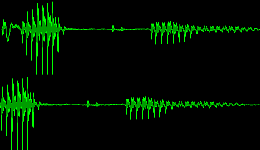
\includegraphics[width=7cm]{bilder/sal0}}
\label{wtd}
\end{minipage}
\end{center}

\vspace{7cm}
\noindent
\begin{center}
\begin{tabular}{r l}
Tutor & Brünig\\
Durchführung & 12. Juni 2013 von 14-18 Uhr \\

E-Mail Dominik & dominik.wille@fu-berlin.de \\
E-Mail Alexander & Matthias.Heinisch@gmx.de \\
\end{tabular}
\end{center}

\newpage
\tableofcontents
\newpage

\section{Physikalische Grundlagen}
\subsection{Schallwellen und Ausbreitungsgeschwindigkeit}
Tritt eine zunächst lokale Erregung in einem ausgedehnten, elastischen Medium auf, entsteht eine Welle, welche sich räumlich ausbreitet. Die Geschwindigkeit, mit der sich diese Erregung ausdehnt, nennt man Phasen-, bzw. Schallgeschwindigkeit und hängt von der Rückstellkraft und der Trägheit des Mediums ab. Es gilt:

\begin{equation}
\label{c}
c=\sqrt{\frac{D}{\rho}}
\end{equation}

Mit der Rückstellkonstanten D und der Dichte \(\rho\).\\
Nimmt man nun einen Festkörper als Medium, besitzt in diesem jedes Volumenelement eine fest definierte Ruheposition. Nun unterscheidet man zwischen zwei Arten von Wellen in diesem Körper. Die Erste ist die longitudinale Dichtewelle, welche in Ausbreitungsrichtung schwingt. Des Weiteren gibt es die transversale Scherwelle. Sie schwingt im Gegensatz zur Longitudinalwelle senkrecht zur Ausbreitungsrichtung, ist nicht an ein Medium gebunden und kann polarisiert werden (z.B. Licht).In Gasen und Flüssigkeiten treten nur Dichtewellen auf, wodurch die Rückstellkonstante durch das Kompressionsmodul K ausgedrückt wird.\\
Da zum einen die Periodendauer von Schallwellen in Gasen relativ kurz ist, und zum anderen Gase eine geringe Wärmeleitfähigkeit besitzen, findet kein Energieaustausch zwischen den einzelnen Teilchen statt. Damit gilt die Poisson-Gleichung:

\begin{equation}
\label{rho}
\rho \cdot V^{\kappa} = const.
\end{equation}

welche durch Ableiten einen Ausdruck für die Kompressionsrate K liefert:

\begin{equation}
\label{K}
D = K = V \frac{d\rho}{dV}=-\kappa \rho
\end{equation}

mit dem Isentropenindex 

\begin{equation}
\label{kappa}
\kappa = \frac{c_{p}}{c_{v}}
\end{equation}

Daraus folgt für c:

\begin{equation}
c=\sqrt{\kappa\frac{p}{\rho}}=c(T)
\end{equation}

Die Schallgeschwindigkeit ist wegen der Dichte Temperaturabhängig, wobei sie nicht Druckabhängig ist, da sich die Trägheits- und Rückstellgröße im gleichen Maße mit dem Druck ändert.

\newpage
\subsection{Stehende Welle}
\newpage
\section{Aufgaben}
\subsection{Aufgabe 1}
Messung der Schallgeschwindigkeit in Luft durch Laufzeitmessung.
\subsection{Aufgabe 2}
Beobachtung der Resonanzen einer Luftsäule mit abgeschlossenem bzw. offenem Ende durch Variation der Anregungsfrequenz. Berechnung der Schallgeschwindigkeit und des Verhältnisses der spezifischen Wärme \(\frac{c_{p}}{c_{v}}=\kappa\) von Luft (Isentropenindex, Adiabatenkoeffizient).
\subsection{Aufgabe 3}
Bestimmung der Schallgeschwindigkeit in Metallen aus der Laufzeit bzw. der Grundschwingungsfrequenz für zwei verschiedene Einspannungen des Stabes. Berechnung des Elastizitätsmoduls des Metalls.


\end{document}